\documentclass[11pt]{article}
\usepackage{hyperref} 
\usepackage{amsmath, amsfonts, amssymb}
\usepackage{graphicx}
\usepackage{float}
\usepackage[backend=biber,style=ieee,sorting=ynt]{biblatex}
\addbibresource{references.bib} 
\usepackage[margin=1in]{geometry}
\usepackage{booktabs}

\emergencystretch=0pt
\pretolerance=150
\tolerance=10000
\hbadness=10000
\hfuzz=0pt

\title{230ZB Problem Set Writeup}
\author{Angel Chen, Jan-Luca Frick, Brian Jairam, Jack Krupinski, Nathan Ueda}
\date{\today} 

\begin{document}
\maketitle 
\pagebreak
% \tableofcontents 
% \pagebreak

\section{Introduction}
Our strategy utilizes a GICS sector-based approach to select which S\&P constituents 
to long and short. Given an FOMC statement and a prompt, the fine-tuned model chooses 
a single sector to long and a single sector to short. We then construct a long-short 
portfolio from these stocks and hold it for 1 day.

\section{Data}

Since we were limited to data related to S\&P constituents and FOMC statements, 
the data cleaning process was relatively simple. For the FOMC statements, we started 
by converting all PDF statements into their respective URLs so that we had all the 
FOMC statements in a uniform format. We then read each FOMC statement into a dataframe, 
scraped the relevant text, and removed stop words.

    For the S\&P data, we pulled data from CRSP from the start of 2000 to the end of 2023, 
along with the corresponding GICS classification data. It is worth noting that companies may, 
at times, get reclassified into different GICS sectors as their revenue sources change. Since the 
GICS information from CRSP is static, these reclassifications are not accounted for. However, 
the number of reclassified stocks is quite low, so we expect these reclassifications to have 
minimal effect. Accounting for this could be an interesting area for future research.

\section{Methodology}
As mentioned earlier, we provided the GPT model with a prompt and an FOMC statement to 
forecast which sector would have the highest and lowest returns over the next day. We 
then constructed a portfolio to hold for one day.

    OpenAI recommends refining the prompt on a non-fine-tuned model first and only fine-tuning once 
the desired results are achieved. We followed this recommendation by refining our prompt on 
the base model. Once satisfied with the output, we proceeded to fine-tune the model.

    To fine-tune the model, we created a labeled dataset where the input consisted of the FOMC 
statement combined with our prompt, and the label indicated which sectors had the highest 
and lowest returns over the next day. Based on how we framed the objective, this label 
corresponds to the correct answer. An example of what a row of data looked like is:

\begin{verbatim}
{
    "messages": [{
    # system message to describe the chatbot
    "role": "system",
    "content": f"""As of {date.strftime('%Y-%m-%d')}, you are a financial 
    analyst specializing in interpreting FOMC statements to predict GICS sector 
    returns in the stock market."""
},
{   
    # system to describe what we are asking the
    "role": "user",
    "content": f"""Based on the FOMC statement released on {date.strftime('%Y-%m-%d')}, 
    please identify:

    - The sector that will have the highest returns over the next day.
    - The sector that will have the lowest returns over the next day.

    Provide your answer in the following format:
    'long: sector, short: sector'

    Recall the list of sector to choose from are:
    'Energy', 'Materials', 'Industrials', 'Consumer Discretionary', 'Consumer 
    Staples', 'Health Care', 'Financials', 'Information Technology', 'Communication 
    Services', 'Utilities', 'Real Estate' 

    Here is the FOMC Statement:
    \"\"\"
    {statement}
    \"\"\"
    """
},
{
        "role": "assistant", 
        "content": row['strategy']
}
    ]
}
\end{verbatim}

Once we had the fine-tuned model, we used it to output which sectors to long and short, 
and constructed our portfolio accordingly.

Initially, we considered asking the model to forecast sentiment based on the FOMC statements, 
and then long sectors that tend to perform well and short sectors that perform poorly. 
However, after further investigation into the data, we identified several factors that 
motivated our current strategy:

\begin{itemize}
  \item All sectors have a negative mean return on days following the FOMC.
  \item All sectors had multiple instances where they would have been sufficed as a good long 
  or a good short.
\end{itemize}

These observations led us to allow any sector to be long or short based on the model's output, 
rather than restricting the model to forecast sentiment and then long/short sectors accordingly. 
We also experimented with different GICS levels, such as industry group and industry. Ultimately, 
we chose sector-level classification due to the limited data available for training. Using 
finer GICS classifications would ideally require more data points for training.
 

\section{Mitigating Lookahead Bias}
There were many proposed ways of mitigating lookahead bias and listed below are two simple 
options. 
\begin{enumerate}
    \item Date Removal: Removing all mentions of dates of any kind.
    \item Time Based Prompt Engineering: In the prompt, specify that ChatGPT is an analyst that 
    only knows public information up to and including the date of the relevant FOMC statement.
\end{enumerate}

We implement the second method (as seen in the above prompt). Time-based prompt engineering
attempts to reduce lookahead bias by anchoring the model's perspective to a specific date. 
That being said, there are several issues limit its effectiveness:

\begin{enumerate}
    \item Model's Pretrained Knowledge Beyond Specified Date: The model inherently knows about events after the specified date due to pretraining on extensive datasets, making it challenging to restrict responses to past information.
    
    \item Implicit Knowledge and Associations: Learned associations spanning across time might cause the model to include future information or trends inadvertently.
    
    \item Difficulty in Enforcing Temporal Constraints: Without an internal representation of time, the model cannot inherently enforce temporal boundaries in its responses.
    
    \item Risk of Hallucinations: To comply with temporal constraints, the model might generate plausible but fabricated information, leading to inaccuracies.
    
    \item Inconsistent Behavior: The model's adherence to temporal instructions can be unpredictable, resulting in inconsistent mitigation of lookahead bias.
\end{enumerate}

While some lookahead bias may persist despite instructing the model not to use post-event data, 
the complexity of our task further mitigates this bias. Unlike simple yes/no questions, 
predicting which sector will perform the best and worst requires intricate knowledge of:

\begin{enumerate}
    \item S\&P 500 Constituents: The model would need to know the current constituents of the index as of the prediction date, not afterward.
    \item GICS Classifications: Correctly identifying which sectors specific companies belong to adds another layer of complexity.
    \item Market Dynamics: Short-term market movements are driven by many unpredictable factors, making it difficult for residual lookahead bias to provide definitive answers.
    \item Uncertainty: Market predictions are inherently uncertain, even for experts, reducing the likelihood that lookahead bias could fully determine the correct sectors.
\end{enumerate}

Thus, the complexity of this task helps limit the impact of residual lookahead bias. Additionally, 
an indicator of significant realized lookahead bias could be very high accuracy. However, our 
model's accuracy is modest, which suggests that lookahead bias is not a dominant factor. For longs, 
the accuracy was 12.8\%, for shorts 20.5\%, and overall accuracy was 16.7\%. Although these numbers 
are low, positive returns indicate that the model's forecasts were close enough to the actual 
market moves to generate positive returns.


%%
\section{Results}

Below, we present the summary statistics for the returns of each portfolio constructed at the close of each FOMC statement and held for one day. The table provides key insights into the performance distribution of our portfolios based on the long-short sector strategy recommended by the fine-tuned GPT model.

\begin{table}[H]
\centering
\begin{tabular}{lr}
\toprule
\textbf{Statistic} & \textbf{Value} \\
\midrule
Mean          & 0.001940       \\
Std           & 0.023244       \\
Min           & -0.064952      \\
25\%          & -0.007146      \\
50\% (Median) & 0.000204       \\
75\%          & 0.008981       \\
Max           & 0.103960       \\
\bottomrule
\end{tabular}
\caption{Summary Statistics for \texttt{position\_return}}
\end{table}

\begin{itemize}
    \item Mean Return: On average, the portfolios provided a small positive return of 0.194\%. While the return may seem modest, this strategy aims to capture short-term market inefficiencies, and cumulative returns over time may result in more significant gains.
    \item Standard Deviation: The standard deviation of 0.0232 indicates moderate volatility in daily returns. As expected with a long-short strategy, the vol is kept within reasonable bounds.
    \item Minimum and Maximum Returns: The range of returns varies from a minimum of -6.5\% to a maximum of 10.4\%. This highlights the potential for both gains and losses during highly volatile market periods, such as after FOMC statements.
\end{itemize}


After accounting for each FOMC statement, the Sharpe ratio for the portfolio stands at 1.32. A Sharpe ratio of 1.32 implies that the strategy generates good returns relative to the risk taken, especially for short-term trading strategies.

To gain further insights into the portfolio construction, we also analyzed the sectors selected by the model for long and short positions during the test period.

\begin{table}[H]
\centering
\begin{tabular}{lr}
\toprule
\textbf{Sector} & \textbf{Count} \\
\midrule
Real Estate           & 23 \\
Utilities             & 9  \\
Consumer Discretionary & 5  \\
Energy                & 2  \\
\bottomrule
\end{tabular}
\caption{Sector Counts for Long Positions}
\end{table}

\begin{table}[H]
\centering
\begin{tabular}{lr}
\toprule
\textbf{Sector} & \textbf{Count} \\
\midrule
Energy                 & 27 \\
Information Technology & 9  \\
Utilities              & 2  \\
Real Estate            & 1  \\
\bottomrule
\end{tabular}
\caption{Sector Counts for Short Positions}
\end{table}

\subsubsection*{Sector Performance Interpretation}
\begin{itemize}
    \item Energy as a Short: The model consistently selected Energy as a short position 27 times, which likely reflects its perceived vulnerability or negative reaction to FOMC decisions during the test period. This heavy weighting toward Energy as a short may indicate that the sector was particularly sensitive to rate hikes or macroeconomic uncertainty caused by the FOMC announcements.
    
    \item Real Estate as a Long: The model's preference for Real Estate as a long position (23 times) suggests that this sector may have been seen as more resilient or capable of benefiting from the market environment following FOMC announcements. Given that real estate investments are often considered more stable or a hedge against inflation, this could explain its frequent selection.
    
    \item Balanced Selection for Information Technology: While Information Technology was chosen both as a long and short sector, its relatively lower frequency suggests that the model didn’t have as strong a directional bias for this sector, likely due to mixed market reactions to FOMC announcements during the period.
\end{itemize}

\subsubsection*{Cumulative Returns}
The following figure shows the cumulative returns of the strategy over the test period. The cumulative performance of the portfolio was doing well until the second half of 2022, after which there was a noticeable decline. This drop coincides with increased market volatility, possibly due to the changing macroeconomic environment and tightening of monetary policy by the Federal Reserve.

\noindent 
\begin{figure}[H] 
  \centering 
  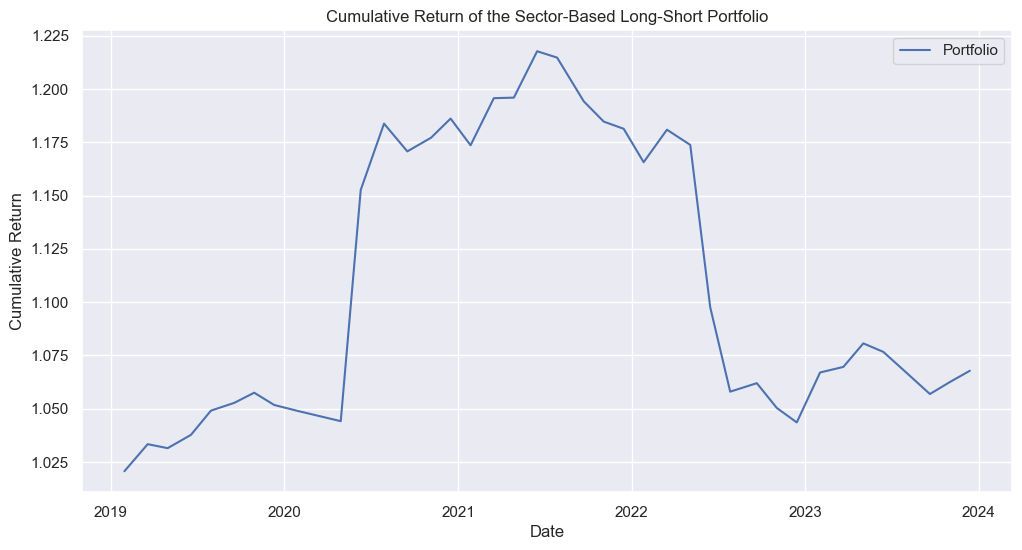
\includegraphics[width=5.2in]{imgs/cum_ret.png}
  \caption{Cumulative Returns}
\end{figure}

\begin{itemize}
    \item The strategy performed consistently well until the middle of 2022, showing steady gains.
    \item The decline starting in the second half of 2022 could be attributed to heightened uncertainty in the market, changes in interest rate policy, and possible shifts in the sectors that historically reacted predictably to FOMC announcements.
    \item The positive cumulative returns, despite the challenges in late 2022, suggest that the model was able to capture short-term opportunities in the market effectively, even though it faced challenges adapting to new market conditions.
\end{itemize}

\subsubsection*{Conclusion}
The results indicate that our GPT-based sector selection strategy was successful in generating positive returns over the test period. The positive Sharpe ratio and cumulative returns demonstrate the effectiveness of the strategy, although there are opportunities to refine the model, particularly in adapting to shifting market conditions during periods of increased volatility (as seen in late 2022).

Future work could explore improving the model's adaptability to changing market dynamics, as well as incorporating additional data sources or factors that could provide further insights into sector performance following FOMC announcements.

\end{document}
